\subsection{角的分类}\label{subsec:czjh1-1-8}

根据角的大小,我们可以将角分成不同的类。

如图 \ref{fig:czjh1-1-34},射线 $OB$ 是平角 $\angle AOC$ 的平分线。
即 $\angle AOB = \angle BOC = \exdfrac{1}{2} \angle AOC$。

\begin{figure}[htbp]
    \centering
    \begin{minipage}[b]{5cm}
        \centering
        \begin{tikzpicture}
	\tkzDefPoints{0/0/O, -1.5/0/A, 1.5/0/C, 0/1.5/B}
	\tkzDrawSegments(O,A  O,B  O,C)
	\tkzMarkRightAngle(B,O,C)
	\tkzLabelPoints[right](B)
	\tkzLabelPoints[below](A, O, C)
\end{tikzpicture}


        \caption{}\label{fig:czjh1-1-34}
    \end{minipage}
    \qquad
    \begin{minipage}[b]{9cm}
        \begin{minipage}[b]{4cm}
            \centering
            \begin{tikzpicture}
	\tkzDefPoints{0/0/O, 1.5/0/A, 1.1/1.5/B, 0/1.5/M}
	\tkzDrawSegments(O,A  O,B)
	\tkzDrawSegments[dashed](O,M)
	\tkzMarkRightAngle(M,O,A)
	\tkzLabelPoints[right](B)
	\tkzLabelPoints[below](A, O)
\end{tikzpicture}


            \caption*{甲}
        \end{minipage}
        \qquad
        \begin{minipage}[b]{4cm}
            \centering
            \begin{tikzpicture}
	\tkzDefPoints{0/0/Q, 1.5/0/C, -1.0/1.5/D, 0/1.5/M, -1.0/0/N}
	\tkzDrawSegments(Q,C  Q,D)
	\tkzDrawSegments[dashed](Q,M  Q,N)
	\tkzMarkRightAngle(M,Q,C)
	\tkzLabelPoints[left](D)
	\tkzLabelPoints[below](C, Q)
\end{tikzpicture}


            \caption*{乙}
        \end{minipage}
        \caption{}\label{fig:czjh1-1-35}
    \end{minipage}
\end{figure}

当一个角等于平角的一半时,这个角叫做\zhongdian{直角}。
图 \ref{fig:czjh1-1-34} 中的 $\angle AOB$ 、$\angle BOC$ 都是直角。
直角可以用 $Rt \angle$ 表示。记作 $\angle AOB = Rt \angle$ 或 $Rt \angle AOB$。
图中角顶处的符号 “\tikz \draw(0,0)--(1.5ex,0) -- (1.5ex,-1.5ex);” 表示这个角是直角。

因为直角是平角的一半,所以
{\bfseries
\begin{align*}
    & \bm{1 \text{周角} = 4 \text{直角;}} \\
    & \bm{1 \text{平角} = 2 \text{直角;}} \\
    & \bm{1 \text{直角} = 90^\circ \juhao}
\end{align*}}

因为每个直角都是 $90^\circ$, 所以所有的直角都相等。
小于直角的角叫做\zhongdian{锐角},大于直角而小于平角的角叫做\zhongdian{钝角}。
如图 \ref{fig:czjh1-1-35} 甲中, $\angle AOB < Rt \angle$,所以 $\angle AOB$ 是锐角,
图 \ref{fig:czjh1-1-35} 乙中,$180^\circ > \angle CQD > Rt \angle$,所以 $\angle CQD$ 是钝角。

两个角的和等于直角时,说这两个角\zhongdian{互为余角},简称\zhongdian{互余},也可以说其中一个角是另一个角的\zhongdian{余角}。
两个角的和等于平角时,说这两个角\zhongdian{互为补角},简称\zhongdian{互补},也可以说其中一个角是另一个角的\zhongdian{补角}。
将一个角的一边反向延长,这条反向延长线与这个角的另一边构成一个角,这时说,它和原来的角\zhongdian{互为邻补角}。
如图 \ref{fig:czjh1-1-36} 甲,$\angle 1$ 与 $\angle 2$ 互余,记作 $\angle 1 + \angle 2 = 90^\circ$ 或 $\angle 1 = 90^\circ - \angle 2$;
如图 \ref{fig:czjh1-1-36} 乙,$\angle 3$ 与 $\angle 4$ 互补,记作 $\angle 3 + \angle 4 = 180^\circ$ 或 $\angle 3 = 180^\circ - \angle 4$;
如图 \ref{fig:czjh1-1-36} 丙,$AB$、$CD$ 是两条直线,$\angle 1$ 和 $\angle 2$, $\angle 2$ 和 $\angle 3$ 都互为邻补角。

\begin{figure}[htbp]
    \centering
    \begin{minipage}[b]{4cm}
        \centering
        \begin{tikzpicture}
	\pgfmathsetmacro{\r}{1.5}
	\pgfmathsetmacro{\R}{1.5}
	\pgfmathsetmacro{\a}{30}
	\pgfmathsetmacro{\b}{60}

	\begin{scope} [xshift=-1cm]
		\tkzDefPoints{0/0/B, \r/0/A}
		\tkzDefPoint(\a:\r){C}
		\tkzDrawSegments(B,A  B,C)
		\tkzMarkAngle[size=0.5](A,B,C)
		\tkzLabelAngle[pos=0.8](A,B,C){$1$}
	\end{scope}

	\begin{scope} [xshift=1cm]
		\tkzDefPoints{0/0/B, \r/0/A}
		\tkzDefPoint(\b:\r){C}
		\tkzDrawSegments(B,A  B,C)
		\tkzMarkAngle[size=0.5](A,B,C)
		\tkzLabelAngle[pos=0.8](A,B,C){$2$}
	\end{scope}

	\begin{scope} [yshift=-2cm]
		\tkzDefPoints{0/0/B, \R/0/A}
		\tkzDefPoint(\a:\R){C}
		\tkzDefPoint(\a+\b:\R){D}
		\tkzDrawSegments(B,A  B,C B,D)
		\tkzMarkAngle[size=0.5](A,B,C)
		\tkzLabelAngle[pos=0.8](A,B,C){$1$}
		\tkzMarkAngle[size=0.6](C,B,D)
		\tkzLabelAngle[pos=0.9](C,B,D){$2$}
	\end{scope}
\end{tikzpicture}


        \caption*{甲}
    \end{minipage}
    \qquad
    \begin{minipage}[b]{5cm}
        \centering
        \begin{tikzpicture}
	\pgfmathsetmacro{\r}{1.5}
	\pgfmathsetmacro{\R}{1.5}
	\pgfmathsetmacro{\a}{120}
	\pgfmathsetmacro{\b}{60}

	\begin{scope} [xshift=-1cm]
		\tkzDefPoints{0/0/B, \r/0/A}
		\tkzDefPoint(\a:\r){C}
		\tkzDrawSegments(B,A  B,C)
		\tkzMarkAngle[size=0.5](A,B,C)
		\tkzLabelAngle[pos=0.8](A,B,C){$3$}
	\end{scope}

	\begin{scope} [xshift=1cm]
		\tkzDefPoints{0/0/B, \r/0/A}
		\tkzDefPoint(\b:\r){C}
		\tkzDrawSegments(B,A  B,C)
		\tkzMarkAngle[size=0.5](A,B,C)
		\tkzLabelAngle[pos=0.8](A,B,C){$4$}
	\end{scope}

	\begin{scope} [yshift=-2cm]
		\tkzDefPoints{0/0/B, \R/0/A}
		\tkzDefPoint(\b:\R){C}
		\tkzDefPoint(\a+\b:\R){D}
		\tkzDrawSegments(B,A  B,C B,D)
		\tkzMarkAngle[size=0.5](A,B,C)
		\tkzLabelAngle[pos=0.8](A,B,C){$4$}
		\tkzMarkAngle[size=0.6](C,B,D)
		\tkzLabelAngle[pos=0.9](C,B,D){$3$}
	\end{scope}
\end{tikzpicture}


        \caption*{乙}
    \end{minipage}
    \qquad
    \begin{minipage}[b]{4cm}
        \centering
        \begin{tikzpicture}
	\tkzDefPoints{0/0/C, -0.5/3/A,  2/0/B, 1.5/3/D}
	\tkzInterLL(C,D)(A,B)   \tkzGetPoint{O}
	\tkzDrawSegments(A,B  C,D)
	\tkzMarkAngle[size=0.4](A,O,C)  \tkzLabelAngle[pos=0.7](A,O,C){$1$}
	\tkzMarkAngle[size=0.6](D,O,A)  \tkzLabelAngle[pos=0.9](D,O,A){$2$}
	\tkzMarkAngle[size=0.4](B,O,D)  \tkzLabelAngle[pos=0.7](B,O,D){$3$}
	\tkzLabelPoints[left](A, C)
	\tkzLabelPoints[right](B, D)
\end{tikzpicture}


        \caption*{丙}
    \end{minipage}
    \caption{}\label{fig:czjh1-1-36}
\end{figure}

\liti 已知 $\angle \alpha = 32^\circ 18' 30''$,求 $\angle \alpha$ 的余角与补角的大小。

\jie $\angle \alpha \text{的余角} = 90^\circ - 32^\circ 18' 30'' = 57^\circ 41' 30''$。

$\angle \alpha \text{的补角} = 180^\circ - 32^\circ 18' 30'' = 147^\circ 41' 30''$。


\liti 已知 $\angle \alpha = \angle \beta$, $\angle \alpha$ 的补角是 $\angle \beta$ 的余角的 3 倍。求 $\angle \alpha$ 的大小。

\jie $\angle \alpha$ 的补角为 $180^\circ - \angle \alpha$, $\angle \beta$ 的余角为 $90^\circ - \angle \beta$,根据题意得
\begin{gather*}
    180^\circ - \angle \alpha = 3(90^\circ - \angle \beta) \juhao  \tag{1}
\end{gather*}

已知
\shangyihang \begin{gather*}
    \angle \beta = \angle \alpha \douhao  \tag{2}
\end{gather*}

将 (2) 式代入 (1) 式,得
\begin{gather*}
    180^\circ - \angle \alpha = 3(90^\circ - \angle \alpha) \juhao  \tag{3}
\end{gather*}

解方程得
$$ \angle \alpha = 45^\circ \juhao $$

上面的推理过程中,由 (1) 式变到 (3) 式是将 (1) 式中的 $\angle \beta$
用与它相等的量 $\angle \alpha$ 来代替,这种等式变形叫做\zhongdian{等量代换}。

图 \ref{fig:czjh1-1-37} 中, $\angle 2$ 与 $\angle 3$ 都是 $\angle 1$ 的余角,下面我们来比较这两个角的大小。

\begin{figure}[htbp]
    \centering
    \begin{tikzpicture}
	\pgfmathsetmacro{\r}{2.5}
	\pgfmathsetmacro{\a}{55}
	\pgfmathsetmacro{\b}{35}

	\begin{scope}
		\tkzDefPoints{0/0/B, \r/0/A}
		\tkzDefPoint(\a:\r){C}
		\tkzDrawSegments(B,A  B,C)
		\tkzMarkAngle[size=0.5](A,B,C)
		\tkzLabelAngle[pos=0.8](A,B,C){$1$}
	\end{scope}

	\begin{scope}[xshift=4cm]
		\tkzDefPoints{0/0/B, \r/0/A}
		\tkzDefPoint(\b:\r){C}
		\tkzDrawSegments(B,A  B,C)
		\tkzMarkAngle[size=0.5](A,B,C)
		\tkzLabelAngle[pos=0.8](A,B,C){$2$}
	\end{scope}

	\begin{scope}[xshift=8cm]
		\tkzDefPoints{0/0/B, \r/0/A}
		\tkzDefPoint(\b:\r){C}
		\tkzDrawSegments(B,A  B,C)
		\tkzMarkAngle[size=0.5](A,B,C)
		\tkzLabelAngle[pos=0.8](A,B,C){$3$}
	\end{scope}
\end{tikzpicture}


    \caption{}\label{fig:czjh1-1-37}
\end{figure}

根据两角互余的定义,有
$$ \angle 1 + \angle 2 = 90^\circ \douhao \quad \angle 1 + \angle 3 = 90^\circ \douhao $$

利用等量代换,得
$$ \angle 1 + \angle 2 = \angle 1 + \angle 3 \juhao $$

根据等式的性质,上式中两边同减去 $\angle 1$,得
$$ \angle 2 = \angle 3 \juhao $$

这样,我们得到了余角的一个性质:

\begin{xingzhi}
    同角(或等角)的余角相等。
\end{xingzhi}

同样可以得到

\begin{xingzhi}
    同角(或等角)的补角相等。
\end{xingzhi}

\begin{lianxi}

\xiaoti{}%
\begin{xiaoxiaotis}%
    \xxt[\xxtsep]{把两块三角板象图甲那样拼在一起,那么三点 $A$、$O$、$B$ 在一条直线上。为什么?}

    \xxt{将 $Rt \angle AOB$ 的一边 $OA$ 反向廷长(图乙), 这时 $\angle BOC$ 是什么角?为什么?}

\end{xiaoxiaotis}


\begin{figure}[htbp]
    \centering
    \begin{minipage}[b]{7cm}
        \centering
        % 绘制三角板的代码复用以前图片中的代码,
% 在显示坐标点时,指定要显示的名字
\begin{tikzpicture}
	\pgfmathsetmacro{\r}{0.3}

	\pgfmathsetmacro{\ab}{2}
	\pgfmathsetmacro{\ac}{\ab * sqrt(3)}
	\tkzDefPoints{0/0/A, \ab/0/B, 0/\ac/C}
	\tkzDefMidPoint(B,C)    \tkzGetPoint{a}
	\tkzDefMidPoint(A,C)    \tkzGetPoint{b}
	\tkzInterLL(A,a)(B,b)   \tkzGetPoint{O}
	\tkzDefCircle[R](O,\r)  \tkzGetPoint{o}
	\tkzDrawPolygon(A,B,C)
	\tkzDrawCircle(O,o)

	\pgfmathsetmacro{\nab}{2.5}
	\tkzDefPoints{0/0/nA, -\nab/0/nB, 0/\nab/nC}
	\tkzDefMidPoint(nB,nC)      \tkzGetPoint{na}
	\tkzDefMidPoint(nA,nC)      \tkzGetPoint{nb}
	\tkzInterLL(nA,na)(nB,nb)   \tkzGetPoint{nO}
	\tkzDefCircle[R](nO,\r)      \tkzGetPoint{no}
	\tkzInterLL(nB,nC)(B,C)     \tkzGetPoint{M}
	\tkzDrawPolygon(nA,nB,nC)
	\tkzDrawCircle(nO,no)

	\tkzLabelPoint[below](A){$O$}
	\tkzLabelPoint[below](B){$B$}
	\tkzLabelPoint[below](nB){$A$}
\end{tikzpicture}


        \caption*{甲}
    \end{minipage}
    \qquad
    \begin{minipage}[b]{7cm}
        \centering
        \begin{tikzpicture}
	\tkzDefPoints{0/0/O, 2.5/0/A, 0/2.5/B, -2.0/0/C}
	\tkzDrawSegments(O,A  O,B)
	\tkzDrawSegments[dashed](O,C)
	\tkzLabelPoints[above](B)
	\tkzLabelPoints[below](A, O, C)
\end{tikzpicture}


        \caption*{乙}
    \end{minipage}
    \caption*{(第 1 题)}
\end{figure}


\xiaoti{已知 $\angle \alpha = 62^\circ 17' 15''$ ,求 $\angle \alpha$ 的余角和补角的度数,并指出它们是锐角还是钝角。}

\xiaoti{如图,$\angle EOC= \angle AOC = \angle BOD = Rt \angle$。
    在图中找出分别与 $\angle AOB$、$\angle BOC$ 互余的角。
    有与 $\angle BOC$ 互补的角吗?图中有邻朴角吗?
}

\begin{figure}[htbp]
    \centering
    \begin{minipage}[b]{7cm}
        \centering
        \begin{tikzpicture}
	\pgfmathsetmacro{\r}{2}
	\pgfmathsetmacro{\a}{35}

	\tkzDefPoints{0/0/O, 2/0/A, 0/2/C, -2/0/E}
	\tkzDefPoint(\a:\r){B}
	\tkzDefPoint(90+\a:\r){D}

	\tkzDrawSegments(O,A  O,B  O,C  O,D  O,E)
	\tkzMarkRightAngle(A,O,C)
	\tkzMarkRightAngle[size=0.3](B,O,D)
	\tkzLabelPoints[right](B, C, D)
	\tkzLabelPoints[below](A, O, E)
\end{tikzpicture}


        \caption*{(第 3 题)}
    \end{minipage}
    \qquad
    \begin{minipage}[b]{7cm}
        \centering
        \begin{tikzpicture}
	\pgfmathsetmacro{\r}{2}
	\pgfmathsetmacro{\a}{60}

	\tkzDefPoints{0/0/O, -2/0/X1, 2/0/X2, 0/-2/Y1,  0/2/Y2}
	\tkzDefPoint(\a:\r){A}

	\tkzDrawSegments(X1,X2  Y1,Y2  O,A)
	\tkzMarkAngle[size=0.5](A,O,Y2)  \tkzLabelAngle[pos=1.1](A,O,Y2){$30^\circ$}

	\tkzLabelPoints[below right](A)
	\tkzLabelPoints[below left](O)
	\tkzLabelPoint[left](X1){西}
	\tkzLabelPoint[right](X2){东}
	\tkzLabelPoint[below](Y1){南}
	\tkzLabelPoint[above](Y2){北}
	\tkzLabelPoint[above, xshift=1em](A){北偏东$30^\circ$}
\end{tikzpicture}


        \caption*{(第 5 题)}
    \end{minipage}
\end{figure}

\xiaoti{互补的两个角能不能都是锐角、钝角、直角? 互余的两个角呢?}

\xiaoti{如图,$OA$ 是表示北偏东 $30^\circ$ 方向的一条射线。仿照这条射线画出表示下列方向的射线:}
\begin{xiaoxiaotis}

    \xxt{北偏东 $50^\circ$;}

    \xxt{北偏西 $60^\circ$;}

    \xxt{南偏西 $10^\circ$;}

    \xxt{南偏东 $25^\circ$;}

    \xxt{东北方向(即北偏东 $45^\circ$);}

    \xxt{西南方向(即南偏西 $45^\circ$)。}

\end{xiaoxiaotis}

\end{lianxi}

